% ===========================================================================
%  Template acadêmico da disciplina — versão LaTeX
%
%  Origem: analise_dados_2026_2/template.md (conteúdo) e
%          analise_dados_2026_2/template.html (apresentação, export do Google Docs)
%
%  Compilação:  latexmk -pdf main.tex
%               (ou Ctrl+Alt+B no VS Code com a extensão LaTeX Workshop)
%
%  Este arquivo contém TODO o conteúdo do template: as seções preservam a
%  redação, a ordem e a hierarquia do original. Os textos são instruções e
%  modelos para o autor substituir — não são o artigo final.
%
%  Numeração de seções, figuras e tabelas é automática: para referenciá-las
%  use \label (prefixos sec:, fig:, tab:) e \ref, nunca números digitados.
%  Decisões de formatação, divergências e pendências: ver README.md.
% ===========================================================================
\documentclass[12pt,a4paper]{article}

% ---------------------------------------------------------------------------
% Codificação e idioma
% ---------------------------------------------------------------------------
\usepackage[utf8]{inputenc}
\usepackage[T1]{fontenc}
\usepackage[brazilian]{babel}
\usepackage{csquotes}

% O HTML usa a fonte "Times". mathptmx (pacote psnfss) fornece o clone Times
% em texto e matemática e está presente em qualquer instalação do TeX Live.
\usepackage{mathptmx}

% ---------------------------------------------------------------------------
% Página
% O HTML não tem regra @page. A área de texto vem de
%   .c48 { max-width:451.4pt; padding:72pt 72pt 72pt 72pt }
% e 451,4 + 2 x 72 = 595,4pt é exatamente a largura de uma folha A4 (595,3pt).
% Adotamos, portanto, A4 com margens de 72pt = 2,54cm em todos os lados.
% ---------------------------------------------------------------------------
\usepackage[a4paper,margin=2.54cm]{geometry}

% ---------------------------------------------------------------------------
% Parágrafos
% No HTML todo texto é justificado, sem recuo de primeira linha (não há
% text-indent) e com 6pt de espaço entre parágrafos (.c30/.c45: padding-top:6pt).
% ---------------------------------------------------------------------------
\setlength{\parindent}{0pt}
\setlength{\parskip}{6pt}

% ---------------------------------------------------------------------------
% Títulos de seção
% Seção    = Times 13pt negrito, 12pt de espaço acima (HTML: .c22/.c46 em .c43)
% Subseção = Times 12pt negrito, 12pt de espaço acima (HTML: .c31/.c7/.c40)
% O ponto depois do número reproduz "1. Introdução"; o \ref continua devolvendo
% apenas o número ("Seção 7.1"), como no texto original.
% ---------------------------------------------------------------------------
\usepackage{titlesec}
\titleformat{\section}{\normalfont\bfseries\fontsize{13pt}{15pt}\selectfont}%
  {\thesection.}{0.5em}{}
\titlespacing*{\section}{0pt}{12pt}{6pt}
\titleformat{\subsection}{\normalfont\bfseries\fontsize{12pt}{14pt}\selectfont}%
  {\thesubsection.}{0.5em}{}
\titlespacing*{\subsection}{0pt}{12pt}{6pt}

% ---------------------------------------------------------------------------
% Legendas de figuras e tabelas
% HTML: legendas em Times 10pt (footnotesize em documento de 12pt), em negrito
% e terminando com ponto ("Figura 1. ...").
% ---------------------------------------------------------------------------
\usepackage{caption}
\captionsetup{font={footnotesize,bf},labelsep=period,skip=6pt}

% ---------------------------------------------------------------------------
% Figuras, texto riscado, links
% ---------------------------------------------------------------------------
\usepackage{graphicx}
\usepackage[normalem]{ulem}  % \sout{: trecho riscado que existe no texto original
\usepackage{xcolor}
\definecolor{corlink}{HTML}{1155CC}  % azul dos links no HTML (.c39)
\usepackage[colorlinks=true,linkcolor=black,citecolor=black,urlcolor=corlink]{hyperref}
\urlstyle{same}  % links em Times, como no HTML (e não em fonte monoespaçada)

% ---------------------------------------------------------------------------
% Blocos recuados (resumo/abstract e o aviso em itálico da seção 2.1)
% ---------------------------------------------------------------------------
\usepackage{changepage}  % adjustwidth

% ---------------------------------------------------------------------------
% Listas
% O HTML recua o 1º nível em 36pt e o 2º em 72pt (.c42/.c50) e usa ◦ nos
% subitens; o marcador padrão do 2º nível no LaTeX é um travessão.
% ---------------------------------------------------------------------------
\setlength{\leftmargini}{36pt}
\setlength{\leftmarginii}{36pt}
\renewcommand{\labelitemii}{\textopenbullet}

% ---------------------------------------------------------------------------
% Tabelas
% O HTML usa colunas de 72,8pt (Modelo) e 58,7pt (demais), com 2pt de
% preenchimento interno. Mantivemos a mesma largura total (~15cm) e o mesmo
% preenchimento, redistribuindo as colunas para que nenhuma palavra transborde
% (ver README.md). L = alinhada à esquerda, C = centralizada.
% ---------------------------------------------------------------------------
\usepackage{array}
\setlength{\tabcolsep}{2pt}
\newcolumntype{L}[1]{>{\raggedright\arraybackslash}p{#1}}
\newcolumntype{C}[1]{>{\centering\arraybackslash}p{#1}}

% ---------------------------------------------------------------------------
% Bibliografia
% As referências vêm de referencias.bib (biblatex + biber, estilo autor-data) e
% são impressas na seção "Referências" por \printbibliography. Cite no texto com
% \cite{chave}, \parencite{chave} ou \textcite{chave}; só as obras citadas
% aparecem na lista.
\usepackage[backend=biber,style=authoryear]{biblatex}
\addbibresource{referencias.bib}
% Formato das citações: SOBRENOME em maiúsculas e vírgula antes do ano
% -> (ANGHINONI et al., 2019) / ANGHINONI et al. (2019).
\renewcommand*{\mkbibnamefamily}[1]{\MakeUppercase{#1}}
\DeclareDelimFormat{nameyeardelim}{\addcomma\space}
%
% Não há equações no template; se precisar, descomente:
% \usepackage{amsmath}

\begin{document}

% ---------------------------------------------------------------------------
% Identificação
% HTML: título 16pt negrito e centralizado; autores 12pt negrito com
% sobrescrito da afiliação; afiliação 12pt; e-mail em Courier New 10pt.
% ---------------------------------------------------------------------------
\begin{center}
  {\fontsize{16pt}{19pt}\selectfont\bfseries
   Título do Artigo Desenvolvido na Disciplina}\\[12pt]
  {\bfseries Nome1 Sobrenome1\textsuperscript{1}, Nome1 Sobrenome2\textsuperscript{1},
   Gabriel Alves\textsuperscript{1}, Maria C. Batista\textsuperscript{1}}\\[12pt]
  {\textsuperscript{1}Departamento de Estatística e Informática – Universidade Federal
   Rural de Pernambuco (UFRPE) – Pernambuco – Brazil}\\[6pt]
  {\footnotesize\texttt{\{nome.sobrenome1, nome.sobrenome2, gabriel.alves,
   maria.cmbatista\}@ufrpe.br}}
\end{center}

% ---------------------------------------------------------------------------
% Resumo e abstract
% HTML: bloco integralmente em itálico, recuado 0,8cm de cada lado
% (.c45: margin-left/right:22.7pt), com "Resumo."/"Abstract." em negrito.
% ---------------------------------------------------------------------------
\begin{adjustwidth}{0.8cm}{0.8cm}
\itshape
\textbf{Resumo.} O resumo deve ser escrito em um único parágrafo e apresentar:
(1) contexto; (2) problema; (3) como o problema é resolvido hoje e o que falta;
(4) qual é a sua proposta para resolver o problema; e (5) resultados obtidos.
Este resumo deve ser escrito em um único parágrafo e conter de 10 a 20 linhas,
aproximadamente.

\textbf{Abstract.} O abstract deve ser a tradulção do resumo em inglês.
\end{adjustwidth}

% ---------------------------------------------------------------------------
% 1. Introdução
% ---------------------------------------------------------------------------
\section{Introdução}\label{sec:introducao}

A introdução deve possuir exatamente a mesma estrutura do resumo. Contudo,
enquanto no resumo cada uma das 5 dimensões (contexto, problema, solução atual,
proposta e resultados) possui de 2 a 4 linhas, aqui cada dimensão deve possuir
de 1 a 2 parágrafos.

Lembre-se que você deve incluir referências para os tópicos que sejam abordados
e explicados a partir da introdução e não apenas na seção de trabalhos
relacionados (SOBRENOME1, A., 2000; SOBRENOME2, B., 2001). A notação deve ser
conforme apresentado na frase anterior, caso tenham dois a 3 autores, a notação
é um pouco diferente (SOBRENOME1, A., SOBRENOME2, B. e SOBRENOME3, C., 2002).
Caso tenha a partir de 4 autores, utiliza-se o primeiro autor seguido de
\emph{et al.} (SOBRENOME1, A. \emph{et al.} 2003).

Evite usar links como referência. Se precisar incluir algum link, dê preferência
a colocar explicitamente no texto (\url{https://abnt.org.br/}) , ou mesmo como
rodapé\footnote{\url{https://www.todamateria.com.br/normas-abnt-trabalhos/}}.
Caso seja necessário incluir uma referência como link, é preciso incluir o
último acesso à página e dar preferência a links que não baixo risco de sair do
ar e que sejam consolidados (como site do uml, ou de uma linguagem de
programação).

Diante desse contexto, este trabalho investiga as seguintes perguntas de
pesquisa.

\textbf{PP1:} Quais condições de tendência e volatilidade aparecem na série de
preços da PETR4 e como elas se distribuem ao longo do período analisado?

Esta pergunta busca caracterizar a diversidade temporal da série da PETR4. Isto
é, identificar quais condições de tendência e volatilidade estão presentes na
amostra, por quanto tempo se mantêm e como se alternam ao longo do período. A
PETR4, ação preferencial da Petrobras, é um ativo conhecido do mercado acionário
brasileiro e apresenta, em uma exploração preliminar dos últimos cinco anos,
valorização do preço de fechamento entremeada por períodos de queda, o que a
torna um caso de interesse para estudos sobre séries de ações. Esse interesse,
porém, não garante que a série seja adequada para análise: como apontam
\textcite{hu_fintsb_2025}, bases de dados de ações frequentemente não contemplam
a variedade de padrões de movimento observados nos mercados
(\textit{Diversity Gap}), e conjuntos com apenas três a cinco anos de dados podem
não representar todos esses padrões. Assim, embora cinco anos sejam adotados
como janela inicial, esse período pode não ser suficiente, o que torna
necessário verificar quais condições de tendência e volatilidade a base de fato
contém e se essa variedade a torna interessante de explorar. Os critérios de caracterização da tendência e da
volatilidade serão definidos e justificados na Seção~\ref{sec:metodo}.

\textbf{PP2:} Como o comportamento da PETR4 se relaciona com o do índice
Ibovespa nos períodos identificados na PP1?

Esta pergunta busca contextualizar o comportamento da PETR4 em relação ao índice
Ibovespa, tomado como referência de mercado, em termos de concordância ou
divergência de tendência, volatilidade e de associação entre os retornos das
duas séries. Isto é, verificar em quais períodos o ativo acompanha o índice e em
quais se afasta dele. Ela complementa o objetivo principal ao situar a
caracterização da PETR4 em um referencial de mercado. A análise respeita limites
claros: a associação entre retornos não implica relação causal, a comparação com
um único índice não representa o mercado como um todo nem outros ativos, e os
resultados não serão usados para avaliar a capacidade preditiva de modelos.

Deve-se ainda dar uma ideia rápida de algum resultado alcançado. Por isso, esta
seção precisa ser ajustada no fim do trabalho. (Alguns trabalhos ainda colocam
um parágrafo indicando as seções do artigo).

\subsection{Objetivos}\label{sec:objetivos}

O objetivo deste trabalho é preparar, de forma reproduzível, uma base de dados
financeiros da PETR4 e do índice Ibovespa e analisar a diversidade temporal das
condições de tendência e volatilidade da PETR4, contextualizando-a pelo
comportamento do Ibovespa e documentando as decisões de preparação e as
limitações da base.

Para alcançar esse objetivo, são definidos os seguintes objetivos específicos:

\begin{itemize}
  \item Delimitar o período, a frequência e as variáveis de interesse e coletar,
    no \textit{Yahoo Finance}, as séries históricas da PETR4 e do índice
    Ibovespa, com janela inicial de cinco anos;
  \item Inspecionar a qualidade, a cobertura e a consistência das séries,
    identificando valores ausentes, inconsistências e observações extremas;
  \item Preparar e transformar os dados, documentando cada decisão de tratamento
    de modo a permitir a reprodução da base;
  \item Caracterizar as condições de tendência e volatilidade presentes na série
    da PETR4 e sua distribuição ao longo do período (PP1);
  \item Comparar o comportamento da PETR4 com o do Ibovespa nos períodos
    identificados, quanto à concordância de tendência e volatilidade e à
    associação entre os retornos (PP2);
  \item Organizar a base resultante e discutir os resultados obtidos e as
    limitações da base e da janela analisada.
\end{itemize}

% ---------------------------------------------------------------------------
% 2. Referencial Teórico
% ---------------------------------------------------------------------------
\section{Referencial Teórico}\label{sec:referencial}

Esta seção deve explicar os assuntos abordados pelo seu trabalho.

\subsection{[Assunto do Problema Resolvido - renomeie essa seção]}%
  \label{sec:assunto-problema}

Explicar como se explicaria em um livro que explique os assuntos relacionados ao
problema que se pretende abordar. Por exemplo, no caso de educação, explicar
conceitos como evasão, retenção etc.

% Aviso em itálico recuado 7,5cm: no HTML é .c52 { margin-left:212.6pt }.
\begin{adjustwidth}{7.5cm}{0pt}
\itshape
Cuidado para não escrever exatamente o que o autor original falou, você precisa
explicar com suas palavras, se foi exatamente o texto original, deixe claro
colocando em itálico (Smith e Jones, 1999).
\end{adjustwidth}

Cuidado para não escrever exatamente o que o autor original falou, você precisa
explicar com suas palavras, se foi exatamente o texto original, deixe claro
colocando em itálico. SE NÃO BOTAR EM ITÁLICO É PLÁGIO \textbf{MESMO COM A
REFERÊNCIA} (Smith e Jones, 1999)!

\subsection{Aprendizado de Máquina}\label{sec:aprendizado-maquina}

Explicar como se explicaria em um livro de Aprendizado de Máquina (Boulic e
Renault, 1991). Focar apenas os algoritmos que serão utilizados no trabalho

% ---------------------------------------------------------------------------
% 3. Trabalhos Relacionados
% ---------------------------------------------------------------------------
\section{Trabalhos Relacionados}\label{sec:trabalhos-relacionados}

\subsection{Diversidade e Padronização na Avaliação de Séries Financeiras}\label{sec:tr-padronizacao}

\textcite{hu_fintsb_2025} partem da constatação de que a avaliação de métodos de
previsão de séries temporais financeiras apresenta três limitações sistêmicas:
não contempla toda a variedade de padrões de movimento dos mercados
(\textit{Diversity Gap}), carece de protocolos unificados que permitam comparar
estudos (\textit{Standardization Deficit}) e ignora restrições da estrutura de
mercado, o que infla os resultados e reduz sua aplicabilidade prática
(\textit{Real-World Mismatch}). O objetivo é propor um \textit{benchmark}
abrangente e prático para essa área, o FinTSB. Para construí-lo, os autores
dividem 15 anos de dados históricos de ações em segmentos não sobrepostos de
250 pregões e classificam as ações de cada segmento, pela taxa de variação
diária, em quatro padrões de movimento: tendência de alta, tendência de baixa,
volatilidade e eventos extremos (\textit{black swan events}); os dados são
anonimizados e normalizados entre as ações a cada dia, para evitar vazamento de
informação futura, resultando em 20 conjuntos de dados, cinco por padrão, cada
um com 300 ações e 250 pregões, divididos em 70\% para treino, 10\% para
validação e 20\% para teste. A avaliação é padronizada em onze métricas de três
dimensões: ordenação, como o coeficiente de informação (\textit{Information
Coefficient}, IC); carteira, como retorno anualizado, volatilidade, perda máxima
e índice de Sharpe; e erro, MSE e MAE. Um \textit{pipeline} unificado, com
camadas de dados, treinamento, simulação histórica (\textit{backtesting}) e
retorno de resultados, incorpora restrições reais, como taxas de transação de
0,1\% e a estratégia de carteira Top$K$-Drop, que limita a rotatividade. A
contribuição do artigo é esse \textit{benchmark}, com a classificação dos padrões
de movimento, o protocolo padronizado de avaliação e a modelagem de restrições
de mercado, acompanhado de uma comparação ampla entre estratégias clássicas,
modelos de aprendizado de máquina, como XGBoost, LightGBM e ARIMA, de
aprendizado profundo, como LSTM, GRU, TCN, \textit{Transformer} e PatchTST, de
aprendizado por reforço, generativos e baseados em grandes modelos de
linguagem. Nos resultados, nenhum método obteve o melhor desempenho nas três
dimensões de métricas, houve grande heterogeneidade mesmo entre modelos de uma
mesma família, e técnicas modernas de aprendizado profundo não superaram de
forma consistente as estratégias quantitativas tradicionais nem os modelos
baseados em árvores; os modelos treinados no FinTSB e testados no índice CSI 300
em 2024, sem novo treinamento, mantiveram desempenho consistente. Os autores
ressaltam ainda que erros de previsão baixos têm pouca correlação com o retorno
efetivo dos investimentos. O artigo não discute limitações do próprio
\textit{benchmark} nem aponta trabalhos futuros específicos. Esse trabalho
evidencia a necessidade de protocolos de avaliação padronizados, diversificados
quanto aos regimes de mercado e próximos das condições reais de negociação,
ponto que se relaciona às fragilidades de protocolo observadas em vários dos
trabalhos discutidos nesta seção. Assim como o presente trabalho, o artigo
avalia a LSTM e a GRU sobre séries temporais financeiras; diferencia-se, no
entanto, por propor uma infraestrutura de avaliação, e não um modelo, com foco
na previsão de retornos para ordenação de ações e construção de carteiras,
enquanto o presente trabalho aborda a previsão de preços como um problema de
regressão, com foco nas redes recorrentes LSTM e GRU.

\subsection{Detecção de Tendências e Mudanças de Regime}\label{sec:tr-tendencia}

\textcite{miot_empirical_2020} abordam a detecção de tendência em séries
temporais ruidosas, característica de especial interesse em aplicações
financeiras, partindo da constatação de que abordagens de filtragem, como as
médias móveis, funcionam bem em retrospecto, mas demoram a identificar mudanças
de tendência, e de que rotular tendências em dados históricos é subjetivo. O
objetivo é investigar empiricamente a eficiência de redes neurais recorrentes
(\textit{Recurrent Neural Networks}, RNNs) padrão como estimadores de tendência
de uso geral. Para isso, os autores definem a tendência como o sinal do termo
de deriva da série e formulam o problema como uma classificação sequência a
sequência em três classes (queda, ausência de tendência e alta), treinando e
validando os modelos em séries simuladas a partir de três dinâmicas --- uma
linha ruidosa por partes, um processo de Ornstein-Uhlenbeck por partes e um
processo com troca markoviana de regimes ---, com conjuntos de treino de 1.000
séries e de validação de 300 séries. Mais de 400 combinações de arquitetura
(RNN simples, LSTM e GRU), hiperparâmetros e dinâmica de treino são avaliadas
com os otimizadores Adam e RMSprop, e as diferenças de desempenho são analisadas
por regressão linear e por \textit{bootstrap} com intervalos de confiança. Entre
as contribuições, os autores mostram que uma RNN simples pode ser interpretada
como uma generalização da comparação de médias móveis, derivam estimadores de
máxima verossimilhança para as dinâmicas consideradas e constroem uma GRU de
referência, comparada com a média móvel, uma rede neural convolucional
(\textit{Convolutional Neural Network}, CNN), os estimadores de máxima
verossimilhança e um modelo oculto de Markov (\textit{Hidden Markov Model},
HMM). Nos resultados, a RNN simples apresentou perdas medianas maiores que a
LSTM e a GRU, com diferença significativa em relação à GRU, enquanto LSTM e GRU
não diferiram de forma significativa; a GRU de referência, por sua vez, obteve
perda mediana de 0,26 contra 0,43 da média móvel, de 0,25 contra 0,58 da CNN e
de 0,30 contra 0,70 do HMM. Como limitações, os autores reconhecem que as
distribuições de retornos das séries simuladas podem diferir bastante das
observadas em ativos reais, que não foi possível chegar a conclusões robustas
sobre a influência da dinâmica de treino e que a dinâmica com troca de regimes
permaneceu difícil para todos os estimadores, além de indicarem que a validação
da abordagem em dados financeiros reais ainda está em andamento. Como trabalhos
futuros, sugerem usar essas RNNs como blocos de construção de estimadores mais
complexos, transferir o aprendizado obtido em dados estilizados para dados reais
e construir estimadores de mercado protegidos contra sobreajuste. Esse trabalho
reforça que as RNNs com portas superam tanto a RNN simples quanto estimadores
clássicos e que LSTM e GRU apresentam desempenho equivalente, o que sustenta a
escolha de estudar ambas as arquiteturas. Assim como o presente trabalho, o
artigo avalia a LSTM e a GRU sobre séries com características financeiras;
diferencia-se, porém, por tratar a detecção de tendência como uma tarefa de
classificação em dados simulados, enquanto o presente trabalho aborda a previsão
de preços como um problema de regressão sobre séries temporais financeiras.

\textcite{hosseini_pattern-based_2025} partem da constatação de que os modelos
de previsão financeira têm dificuldade com a volatilidade e a complexidade dos
mercados, em parte porque dependem de atributos tradicionais, que não capturam
padrões de preço mais elaborados, e têm como objetivo propor um método de
extração de atributos baseado na detecção de padrões de preço para melhorar o
desempenho de modelos de aprendizado profundo na classificação de séries
temporais financeiras. Os autores utilizam dados negócio a negócio do mercado
futuro de permissões de emissão de carbono da União Europeia (\textit{European
Carbon Emission Allowance}, EUA), de janeiro de 2018 a junho de 2023,
reamostrados em intervalos de 15 minutos com os atributos de abertura, máxima,
mínima, fechamento e volume (OHLCV). O método identifica pontos de pivô, máximos
e mínimos marcados sempre que o preço varia ao menos 5\% em relação ao pivô
anterior, agrupa sequências de seis pivôs em padrões e calcula 11 atributos a
partir das razões entre as distâncias de preço desses pivôs, agrupados em
atributos de curto, médio e longo prazo. Esses atributos são acrescentados aos
dados OHLCV, normalizados por variação percentual, e alimentam dois modelos que
combinam uma camada LSTM ou GRU com camadas densas, cujos hiperparâmetros são
otimizados por busca bayesiana; a tarefa é classificar se o preço subirá ou
cairá no intervalo seguinte de 15 minutos, a partir de segmentos de 40
intervalos, equivalentes a um pregão, divididos em 80\% para treino, 10\% para
validação e 10\% para teste. A contribuição do artigo é esse método de detecção
de padrões e extração de atributos, aplicado a um mercado de energia ainda pouco
explorado nesse tipo de estudo e avaliado por um estudo de ablação. Nos
resultados, a inclusão dos atributos propostos elevou a acurácia da LSTM de
52,33\% para 73,42\% e a da GRU de 52,30\% para 73,40\%, com diferença
estatisticamente significativa, enquanto a LSTM com indicadores técnicos
tradicionais, como médias móveis, RSI, MACD e bandas de Bollinger, alcançou
56,09\%; LSTM e GRU tiveram desempenho equivalente, e o estudo de ablação mostrou
que a remoção dos atributos de curto prazo provocou a maior queda de acurácia,
de 73,4\% para 71,3\%. Os autores não discutem limitações e, como trabalhos
futuros, sugerem aplicar o método a outros mercados financeiros e refinar a
extração para capturar padrões mais complexos. Cabe observar, porém, que os
segmentos são embaralhados antes da divisão entre treino, validação e teste, o
que pode levar informação de períodos posteriores ao treinamento, e que os
hiperparâmetros foram otimizados apenas para a LSTM e reaproveitados na GRU.
Esse trabalho ilustra como a extração de atributos derivados da estrutura de
preços pode melhorar o desempenho de redes recorrentes em séries financeiras.
Assim como o presente trabalho, o artigo avalia a LSTM e a GRU sobre séries
temporais financeiras; diferencia-se, no entanto, por tratar a previsão como
uma classificação da direção do preço em dados intradiários de um mercado de
energia e por concentrar sua contribuição na extração de atributos, enquanto o
presente trabalho aborda a previsão de preços como um problema de regressão,
com foco nas redes recorrentes LSTM e GRU.

\textcite{anghinoni_time_2019} partem da constatação de que a natureza
estocástica das séries temporais ainda deixa em aberto muitos problemas de
extração de conhecimento e têm como objetivo estudar as séries a partir de suas
propriedades topológicas, observadas em uma rede complexa gerada com os dados,
em vez do espaço temporal ou espectral usado pelas técnicas tradicionais, para
detectar e prever tendências. O método extrai seis séries de atributos da série
original, os ruídos, os gradientes e as posições relativas entre máximos e
mínimos, cada um em curto e longo prazo, calculados a partir de médias móveis;
esses atributos são normalizados pelo escore Z e discretizados, e cada vetor
distinto torna-se um nó de uma rede em que dias consecutivos são ligados por
arestas. Um algoritmo de detecção de comunidades baseado em modularidade agrupa
os nós, e cada comunidade é rotulada como tendência de alta ou de baixa
conforme a variação média da série nos dias que a compõem; por fim, cinco
classificadores, \textit{Naive Bayes}, árvore de decisão, MLP, SVM e k-NN, são
treinados para prever a tendência de cada dia a partir dos atributos. Os autores
avaliam o método em uma série senoidal artificial com ruído gaussiano e no
índice Bovespa ao longo de 20 anos, suavizado por uma média móvel de cinco dias,
com períodos de 25 e 125 dias para os atributos de curto e longo prazo. A
contribuição do artigo é esse algoritmo não supervisionado de detecção de
tendências por comunidades de redes complexas, que determina automaticamente o
número de padrões e absorve melhor o ruído. Nos resultados com a série
artificial, a acurácia de classificação ficou próxima de 80\% para ruídos
baixos e caiu a 50\% com variância do ruído de 0,20, enquanto a acurácia de
previsão permaneceu em torno de 60\%; no Bovespa, o método identificou 38
comunidades, gerou retornos acumulados positivos em todos os horizontes
testados, ao contrário dos atributos usados isoladamente, e a previsão superou
95\% de acurácia com a árvore de decisão para o período de 25 dias, com
resultados semelhantes ao trocar o algoritmo de detecção de comunidades. Os
autores não discutem limitações e, como trabalhos futuros, sugerem incorporar
séries correlacionadas, como taxa de juros, câmbio, PIB e inflação, para estudar
relações multivariadas, e adaptar o método a outros domínios, como a
agricultura. Cabe observar, porém, que, no Bovespa, a acurácia de previsão é
medida em relação aos rótulos de tendência gerados pelo próprio método sobre a
série suavizada, e não em relação à variação efetiva dos preços. Esse trabalho
ilustra uma representação estrutural alternativa das séries financeiras, em que
padrões temporais são capturados pela topologia de redes complexas. Assim como
o presente trabalho, o artigo analisa séries temporais financeiras com o
objetivo de prever seu comportamento; diferencia-se, no entanto, por tratar a
tendência como uma classificação obtida por detecção de comunidades em redes
complexas, sem empregar redes recorrentes, enquanto o presente trabalho aborda a
previsão de preços como um problema de regressão, com foco nas redes
recorrentes LSTM e GRU.

\textcite{wan_tcdformer_2024} partem da constatação de que os modelos de
previsão baseados na arquitetura \textit{Transformer} perdem desempenho em séries
temporais reais não estacionárias e de que as técnicas usuais de
estabilização, como a normalização e a diferenciação, eliminam parte dessa não
estacionariedade e prejudicam a previsão diante de eventos relevantes, como
crises financeiras ou mudanças de taxas de juros, com o objetivo de incorporar
explicitamente a detecção de pontos de mudança e a modelagem de tendência à
previsão de séries não estacionárias. Para isso, propõem o \textit{Trend and
Change-point Detection Transformer} (TCDformer), no qual um módulo de
aproximação linear local em escala (\textit{Local Linear Scaling Approximation},
LLSA), baseado na transformada \textit{wavelet} discreta de máxima sobreposição
(\textit{Maximal Overlap Discrete Wavelet Transform}, MODWT), detecta e
reconstrói as mudanças abruptas da série; a série reconstruída é então
decomposta em tendência e sazonalidade, sendo a tendência prevista por um
perceptron multicamadas (\textit{Multilayer Perceptron}, MLP) com normalização
reversível e a sazonalidade por um \textit{Transformer} com atenção
\textit{wavelet}, e a previsão final é a soma das duas. Os experimentos usam
seis bases de referência, das quais apenas uma é financeira, a de taxas de
câmbio diárias de oito países entre 1990 e 2016, além de bases de energia
elétrica, tráfego, clima e casos de gripe, divididas em ordem cronológica, com
janelas de 96 passos para prever horizontes de 96 a 720 passos, avaliadas pelo
MSE e pelo MAE. A contribuição do artigo é o modelo TCDformer, que integra
detecção de pontos de mudança, decomposição em tendência e sazonalidade e
atenção \textit{wavelet}, e que também permite identificar eventos relevantes a
partir da concentração de pontos de mudança. Nos resultados, o TCDformer obteve
o melhor desempenho médio nas seis bases, reduzindo o MSE em 47,14\% e o MAE em
32,43\% em relação aos modelos baseados em \textit{Transformer} e em 47,79\% e
28,50\%, respectivamente, em relação aos modelos de estrutura híbrida, como
TimesNet, DLinear e LSTNet; na base de câmbio, alcançou MSE médio de 0,2666 e
MAE médio de 0,3711, e o estudo de ablação mostrou aumento expressivo do erro
sem o módulo de detecção de pontos de mudança. Os autores reconhecem que a
eficácia do modelo depende da qualidade e da completude dos dados históricos e
que ele pode ter dificuldade em extrapolar tendências de longo prazo, e, como
trabalhos futuros, sugerem investigar outros métodos de decomposição em
tendência e sazonalidade e aplicar o TCDformer a outros cenários. Cabe observar,
porém, que a avaliação em dados financeiros se limita à base de taxas de câmbio
e que modelos recorrentes foram excluídos da comparação com base em resultados
de estudos anteriores. Esse trabalho ilustra o tratamento explícito da não
estacionariedade, por meio de pontos de mudança e da decomposição da série, como
etapa de extração de características antes da modelagem. Assim como o presente
trabalho, o artigo trata a previsão de séries temporais, incluindo uma série
financeira, como um problema de regressão; diferencia-se, no entanto, por
propor uma arquitetura baseada em \textit{Transformer} para previsão
multivariada de longo horizonte em domínios variados, sem avaliar redes
recorrentes, enquanto o presente trabalho concentra a análise nas redes
recorrentes LSTM e GRU aplicadas a séries financeiras.

\subsection{Volatilidade, Não Estacionariedade e Relações entre Ativos}\label{sec:tr-volatilidade}

\textcite{biswas_dual_2025} tratam da previsão de preços de ações e da
avaliação de risco, tarefas dificultadas pela não linearidade, pelo ruído e
pelas dependências de longo prazo das séries financeiras, que modelos como o
ARIMA e a LSTM nem sempre capturam, com o objetivo de prever simultaneamente os
preços futuros e métricas de risco das ações da MasterCard e da Visa. Os autores
utilizam dados diários dessas duas empresas, obtidos na plataforma Kaggle, de
junho de 2008 a junho de 2024, com preços de abertura, máxima, mínima,
fechamento e fechamento ajustado, volume, retornos diários e médias móveis; os
valores ausentes são preenchidos com a última observação disponível e os dados
são normalizados pelo método \textit{min-max}. O modelo proposto combina uma
rede convolucional temporal (\textit{Temporal Convolutional Network}, TCN), cujas
convoluções dilatadas capturam dependências de curto e longo prazo, com um
mecanismo de atenção que pondera os passos de tempo mais relevantes, e possui
duas saídas: uma prevê os preços de abertura, fechamento, máxima e mínima, e a
outra prevê a volatilidade e o índice de Sharpe, com uma função de perda que
pondera os dois objetivos. O treinamento usa o otimizador Adam e divisão
temporal, com os hiperparâmetros escolhidos por busca em grade, e o melhor
resultado foi obtido com treino de 2008 a 2018 e teste de 2019 a 2024. A
contribuição do artigo é essa arquitetura TCN com atenção e saída dupla,
apresentada como a primeira a prever conjuntamente preços e métricas de risco.
Nos resultados, o modelo obteve MAE de 1,23 para a MasterCard e de 1,45 para a
Visa, com $R^2$ de 0,95 e 0,93, contra MAE de 1,40 e 1,60 da LSTM, de 1,50 e 1,70
do ARIMA e de 1,35 e 1,55 de um modelo baseado em \textit{Transformer}, além de
superar variantes da TCN com outros mecanismos de atenção e sem atenção; na
previsão de risco, alcançou MAE de 0,012 para a volatilidade e de 0,065 para o
índice de Sharpe, e, no \textit{backtesting} e em um experimento adicional com
ações do mercado norte-americano, como Apple e Tesla, manteve desempenho
semelhante. Os autores reconhecem que o modelo usa apenas preços e métricas de
risco, sem fatores externos como indicadores macroeconômicos e sentimento de
notícias, que o equilíbrio entre os dois objetivos pode ser difícil quando
eles conflitam e que a avaliação se limita a duas empresas do mesmo setor; como
trabalhos futuros, sugerem incorporar fontes externas de dados, aplicar técnicas
de otimização multiobjetivo e testar o modelo em outros instrumentos
financeiros. Cabe observar, porém, que o artigo não descreve a configuração da
LSTM e do ARIMA usados como referência e que os mesmos valores de MAE são
apresentados ora como resultado de validação, ora como resultado de teste, o que
dificulta a interpretação dos resultados. Esse trabalho ilustra o uso de
mecanismos de atenção associados a arquiteturas convolucionais temporais como
alternativa às redes recorrentes na previsão financeira. Assim como o presente
trabalho, o artigo trata a previsão de preços de ações como um problema de
regressão e compara seu modelo com a LSTM; diferencia-se, no entanto, por propor
uma arquitetura convolucional com atenção e saída dupla, sem considerar a GRU,
enquanto o presente trabalho concentra a análise nas redes recorrentes LSTM e
GRU.

\textcite{anbaee_farimani_adaptive_2024} partem da constatação de que o
comportamento dos investidores é influenciado por múltiplas fontes de
informação, como análise técnica, notícias e sentimento, o que torna as séries
de preços não estacionárias e leva a maioria dos modelos de aprendizado profundo
a prever apenas a direção do preço, com o objetivo de propor um modelo adaptativo
de regressão de preços que integre essas fontes e lide com a não
estacionariedade. Os autores utilizam dados horários de ao menos três anos de
cinco ativos, os pares cambiais EUR/USD, GBP/USD e USD/JPY, o ouro (XAU/USD) e o
\textit{bitcoin} (BTC/USDT), com preços de abertura, máxima, mínima, fechamento
e volume, indicadores técnicos selecionados para cada ativo e notícias
especializadas sobre cada mercado, divididos em 60\% para treino, 20\% para
validação e 20\% para teste. As notícias são representadas por um método baseado
em conceitos econômicos latentes, obtidos pelo agrupamento de representações
contextuais do BERT com o \textit{k-means}, e o sentimento das manchetes é
estimado pelo FinBERT e agregado por hora; a sequência de notícias é processada
por uma rede convolucional recorrente, e as séries de sentimento e de mercado,
por camadas LSTM. Na camada de fusão, o modelo normaliza cada modalidade conforme
sua distribuição estimada na janela, pondera a importância de cada uma e aprende
o desvio do preço em torno da média da janela, que é somado a essa média na
desnormalização. A contribuição do artigo é esse modelo de fusão adaptativa, que
combina conteúdo das notícias, sentimento e indicadores técnicos e considera a
mudança na distribuição dos dados a cada janela. Nos resultados, o modelo
reduziu o MAPE em relação aos modelos de comparação em até 54,95\% no EUR/USD,
63,61\% no USD/JPY, 66,69\% no XAU/USD e 52,90\% no BTC/USDT, com diferenças
estatisticamente significativas pelo teste de Wilcoxon; o estudo de ablação
mostrou que o uso conjunto das três modalidades supera o uso de apenas uma ou
duas, que a representação por conceitos supera a representação do BERT e que a
normalização adaptativa supera a normalização pelo escore Z, e uma estratégia
de negociação simulada no \textit{bitcoin} obteve lucro superior ao do melhor
modelo de comparação. Na análise de erros, os autores reconhecem que o modelo
que usa apenas dados de mercado tende a replicar movimentos já ocorridos e que o
modelo proposto ainda depende de dados de mercado altamente correlacionados,
sendo necessário modelar o sentimento como um processo markoviano, além de
exigir cerca de 62\% mais tempo de treinamento que o modelo de comparação mais
rápido; como trabalhos futuros, propõem aprimorar essa modelagem do sentimento e
treinar um agente de negociação baseado em notícias com aprendizado por reforço
(\textit{Deep Q-Network}). Esse trabalho ilustra a integração de notícias,
sentimento e indicadores técnicos em um modelo de regressão de preços que
emprega a LSTM e trata explicitamente a não estacionariedade das séries. Assim
como o presente trabalho, o artigo trata a previsão de preços como um problema
de regressão sobre séries temporais financeiras e emprega a LSTM; diferencia-se,
no entanto, por usá-la como componente de uma arquitetura multimodal com fusão
adaptativa, em dados horários de câmbio, ouro e criptomoedas, sem considerar a
GRU, enquanto o presente trabalho concentra a análise nas redes recorrentes
LSTM e GRU.

\textcite{luo_short-term_2024} tratam da previsão de curto prazo da correlação
entre ações, essencial para a gestão de carteiras e a diversificação de risco,
partindo da constatação de que os modelos de séries temporais existentes
consideram apenas o histórico das ações e ignoram que a correlação é afetada
por múltiplos fatores e segue tendências instáveis, com o objetivo de melhorar a
precisão dessa previsão. Os autores utilizam dados diários de oito ações do
mercado acionário chinês, divididas em dois grupos de quatro, entre janeiro de
2017 e janeiro de 2022, totalizando 1.227 pregões, com dados de exposição a
fatores fornecidos por uma corretora e dados de negociação de mercado. Os
fatores de risco do modelo Barra, como capitalização de mercado, lucros,
crescimento e alavancagem, são tratados quanto a valores extremos e ausentes,
padronizados e neutralizados, e um modelo multifatorial explica os retornos e
permite calcular a correlação entre as ações. O modelo proposto,
CNN-BiLSTM-\textit{Attention} (CLATT), recebe as séries de correlação e de
retornos, com janela de 68 dias escolhida experimentalmente: a CNN extrai
características de alta dimensão, uma LSTM bidirecional (BiLSTM) de duas
camadas captura as dependências temporais locais e globais, e um mecanismo de
atenção pondera as saídas da BiLSTM; o treinamento usa a função de perda MSE, e
os dados são divididos em 80\% para treino e 20\% para teste. A contribuição do
artigo é o modelo CLATT, associado ao uso de um modelo multifatorial para
quantificar a correlação e à inclusão dos retornos como entrada adicional,
comparado com CNN, LSTM, CNN-LSTM e CNN-BiLSTM pelas métricas MSE, RMSE, MAE,
MAPE e $R^2$. Nos resultados, o CLATT obteve $R^2$ de 0,9825 e 0,9661 nos dois
grupos, contra 0,9577 e 0,9184 da LSTM e 0,9647 e 0,9329 da CNN-BiLSTM, e
reduziu o MAPE em 57,32\% e 33\% em relação à LSTM e em 56,06\% e 28,87\% em
relação à CNN-BiLSTM; o estudo de ablação mostrou que incluir os retornos como
entrada reduz os erros em relação ao uso exclusivo das séries de correlação. Os
autores reconhecem que a natureza caótica do sistema financeiro ainda limita a
precisão, que os fatores considerados poderiam ser mais abrangentes e que, por
restrições de tempo e de dados, não usaram ações de outros mercados, e indicam
esses pontos como trabalhos futuros. Cabe observar, porém, que a avaliação usa
apenas oito ações de um único mercado e que o artigo não informa se a divisão
entre treino e teste respeita a ordem cronológica. Esse trabalho ilustra a
combinação de convoluções, redes recorrentes bidirecionais e mecanismos de
atenção para modelar relações temporais e estruturais entre ativos. Assim como o
presente trabalho, o artigo trata uma tarefa de regressão sobre séries
temporais financeiras e compara seu modelo com a LSTM; diferencia-se, no
entanto, por prever a correlação entre ações, e não seus preços, com uma
arquitetura híbrida que combina CNN, BiLSTM e atenção, sem considerar a GRU,
enquanto o presente trabalho concentra a análise nas redes recorrentes LSTM e
GRU.

% ---------------------------------------------------------------------------
% 4. Método
% ---------------------------------------------------------------------------
\section{Método}\label{sec:metodo}

Nesta seção, deve-se seguir o KDD, explicando o que será feito em cada etapa do
processo, considerando o seu trabalho específico.

Cada subseção desta seção~\ref{sec:metodo}, deve ser referente a uma etapa do
KDD.

\subsection{Etapa 1}\label{sec:etapa-1}

Explicar a etapa 1 do kdd aplicada ao seu trabalho.

\subsection{Etapa 2}\label{sec:etapa-2}

Explicar a etapa 2 do kdd aplicada ao seu trabalho.

% ---------------------------------------------------------------------------
% 5. Análise Exploratória
% ---------------------------------------------------------------------------
\section{Análise Exploratória}\label{sec:analise-exploratoria}

Esta seção deve apresentar os resultados das análises realizadas sobre os dados.
Mostrar os dashboards e gráficos criados, conforme Figura~\ref{fig:eda}. Observe
que a referência à figura foi feita com letra maiúscula e de forma explícita no
texto. Não deve usar estratégias como ‘A figura abaixo:’. A legenda deve
finalizar com um ponto. Caso a figura não seja sua, inclua a fonte (caso seja
sua, pode-se incluir ‘Fonte: o autor.’). Cuidado caso a imagem não seja sua,
para que não haja nenhum copyright que o proíba a sua inclusão em outros
trabalhos, mesmo com a fonte.

\begin{figure}[htbp]
  \centering
  % No HTML esta legenda é centralizada (.c54); as demais são justificadas.
  \captionsetup{justification=centering}
  % Largura de exibição do HTML: 361,90px = 9,54cm.
  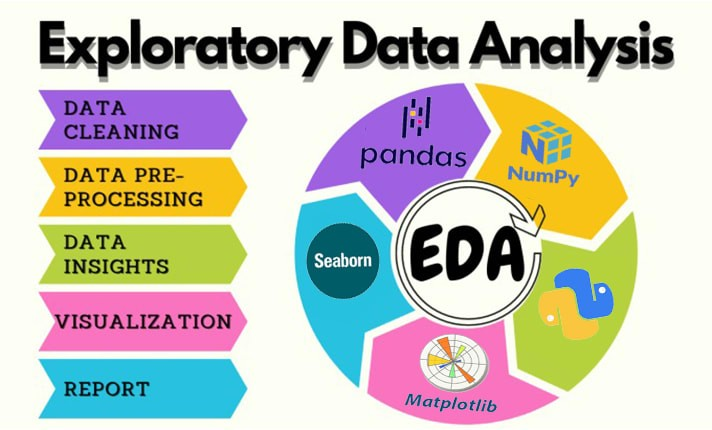
\includegraphics[width=9.54cm]{figuras/eda.png}
  \caption{Uma figura sobre o assunto. \normalfont Fonte:
    \url{https://www.linkedin.com/pulse/preparing-data-eda-mahsa-salimi-2859f/}}
  \label{fig:eda}
\end{figure}

Na EDA, deve-se detalhar as análises e não apenas gerar gráficos. Aqui deve-se
ter indícios iniciais que ajudarão a responder às perguntas de pesquisa, ou
mesmo auxiliar na criação dos modelos de ML.

% ---------------------------------------------------------------------------
% 6. Aplicativo Flutter
% ---------------------------------------------------------------------------
\section{Aplicativo Flutter}\label{sec:aplicativo}

Esta seção deve mostrar o app.

\subsection{[Pergunta de pesquisa 3 - reescrever aqui]}\label{sec:pergunta-3}

Explicar aqui como seu app responde à pergunta de pesquisa 3. Cuidado com o que
prometeu nos objetivos e na pergunta de pesquisa.

% ---------------------------------------------------------------------------
% 7. Resultados e Discussão
% ---------------------------------------------------------------------------
\section{Resultados e Discussão}\label{sec:resultados}

Esta seção deve discutir com profundidade os resultados do trabalho. Deve-se ter
duas subseções específicas, uma para cada pergunta de pesquisa.

\subsection{[Escrever a primeira pergunta de pesquisa como uma pergunta é válido,
  ou devo escrever como uma afirmação?]}\label{sec:primeira-pergunta}

Aqui deve-se apresentar o passo a passo do trabalho realizado e em seguida
discutir os resultados e como a pergunta de pesquisa foi respondida pelos dados
apresentados. Geralmente, essa primeira pergunta de pesquisa estará associada à
clusterização. Apresentar os clusters criados, os critérios usados para definir
a quantidade de clusters e a característica de cada cluster.

ATENÇÃO PARA DISCUTIR E APRESENTAR:

\begin{itemize}
  \item Cotovelo e Silhueta para KMeans;
  \item Se testar outros algoritmos além do KMeans, explicitar;
  \item Ter atenção para atributos categóricos;
  \item Realizar normalização e padronização;
\end{itemize}

% No HTML os quatro painéis ficam no mesmo parágrafo e quebram em três linhas;
% as larguras abaixo (px -> cm na proporção 1px = 0,75pt) reproduzem essa quebra.
\begin{figure}[htbp]
  \centering
  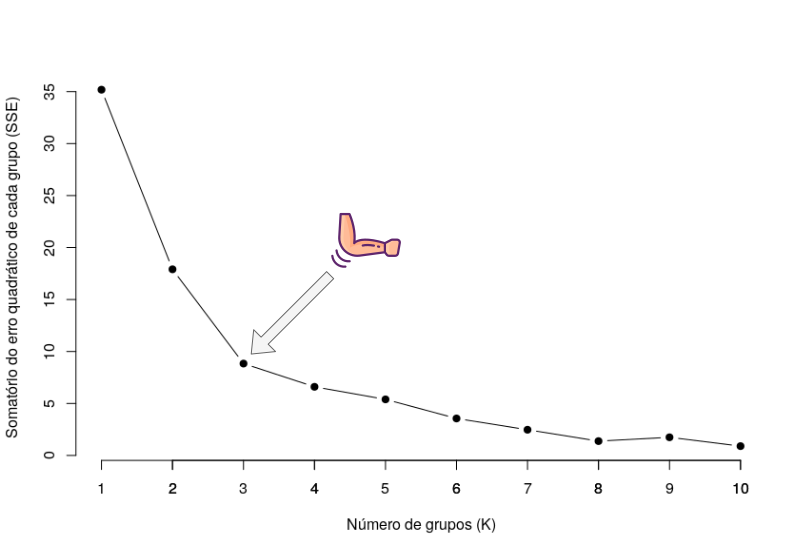
\includegraphics[width=4.36cm]{figuras/cotovelo.png}\hspace{0.4cm}%
  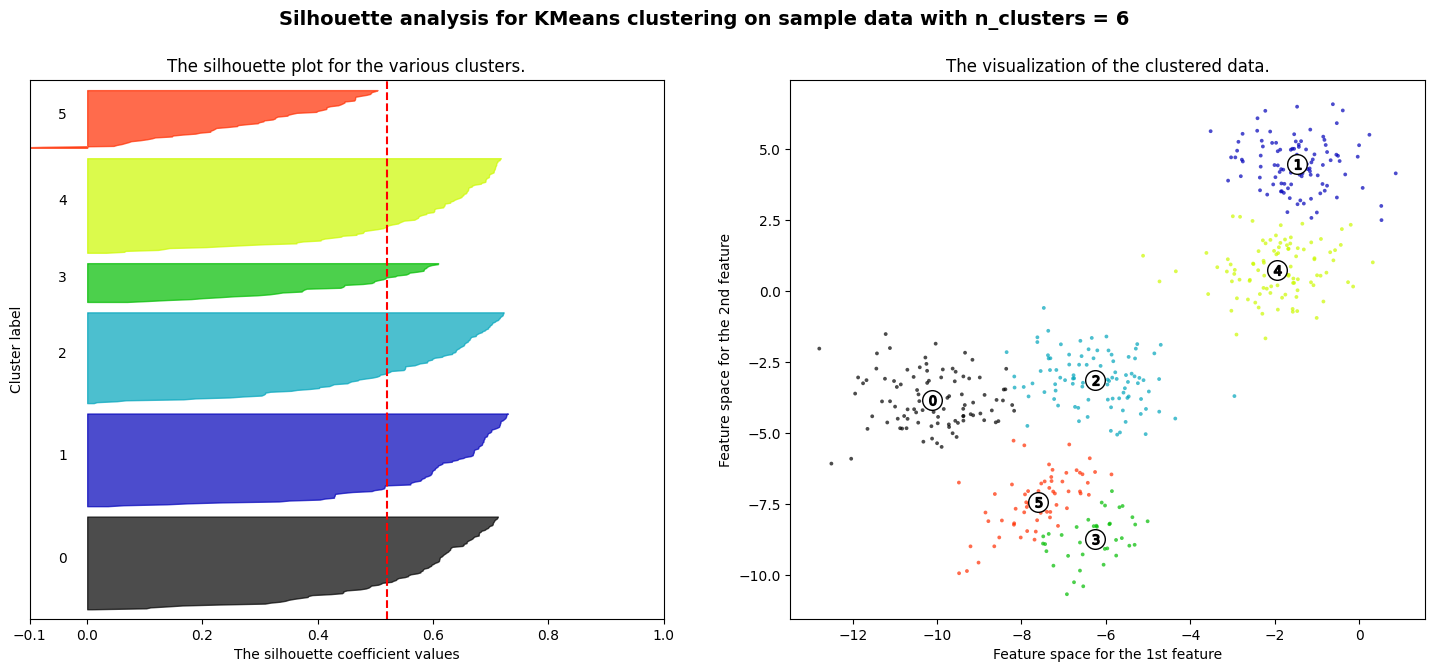
\includegraphics[width=6.07cm]{figuras/silhueta-6-clusters.png}\\[0.3cm]
  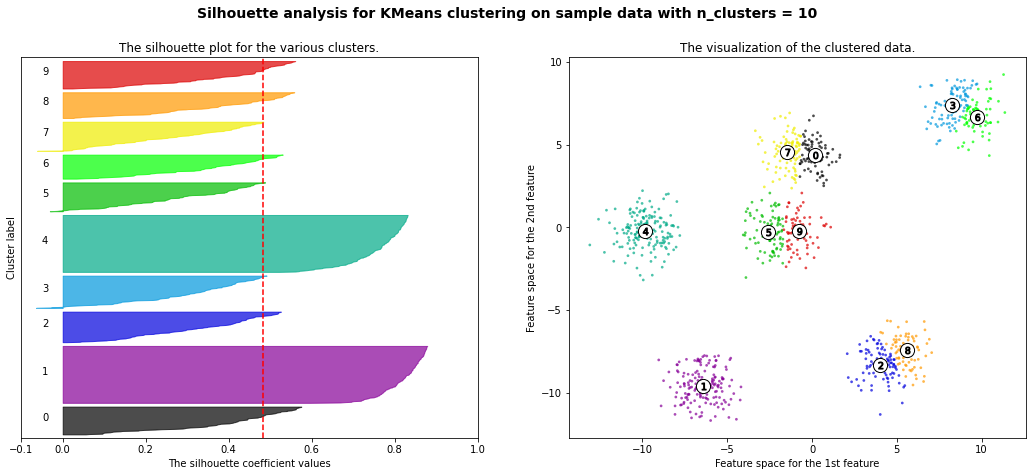
\includegraphics[width=6.92cm]{figuras/silhueta-10-clusters.png}\\[0.3cm]
  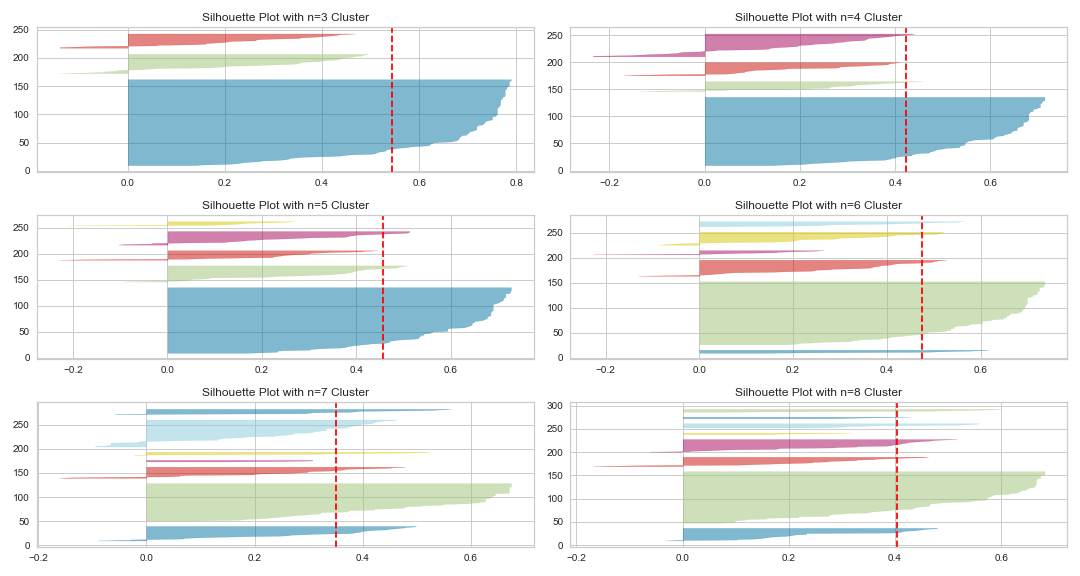
\includegraphics[width=14.94cm]{figuras/silhueta-3-a-8-clusters.png}
  \caption{Método do cotovelo e da silhueta para determinar a quantidade de
    grupos “ideal” no KMeans.}
  \label{fig:cotovelo-silhueta}
\end{figure}

\begin{figure}[htbp]
  \centering
  % Largura de exibição do HTML: 420,88px = 11,09cm.
  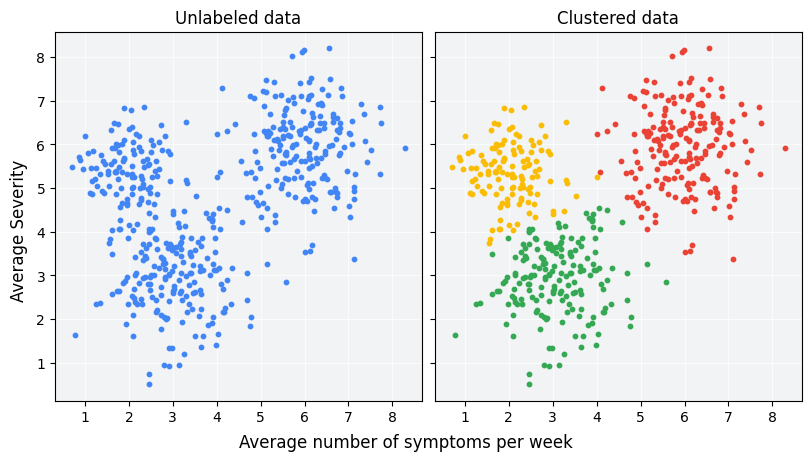
\includegraphics[width=11.09cm]{figuras/dados-clusterizados.png}
  \caption{Dados da nota na 1VA associada à probabilidade de aprovação na
    disciplina. à esquerda os dados originais e à direita os dados
    clusterizados.}
  \label{fig:dados-clusterizados}
\end{figure}

\subsection{[escrever a segunda pergunta de pesquisa]}%
  \label{sec:segunda-pergunta}

Seguir as mesmas orientações dadas para a Seção~\ref{sec:primeira-pergunta}, mas
agora focando a resposta da segunda pergunta de pesquisa. Geralmente, essa
pergunta estará relacionada à classificação. Assim, cabe incluir uma tabela com a
comparação dos resultados, como mostra a Tabela~\ref{tab:resultados-treino}. A
Tabela~\ref{tab:resultados-treino} mostra valores fictícios que devem ser usados
para discutir os resultados DO TREINO. Mas, o que vale mesmo são os resultados da
Tabela~\ref{tab:resultados-teste}. Contudo, caso haja uma diferença significativa
entre os resultados de ambas, já há um indicativo de \emph{overfitting}.

Crie uma tabela no Google Sheets e em seguida copie e cole ela nesse documento.
Na caixa de diálogo, indique a vinculação dos objetos. Assim, quando você
atualizar a tabela do Sheets, ela será atualizada aqui.

% Tabela 1 — resultados do treino (valores fictícios, iguais aos da Tabela 2 no
% documento original: foram preservados como estão). Células em negrito seguem
% o original; a coluna Modelo fica vazia nas linhas de continuação, como no HTML.
\begin{table}[htbp]
  \caption{[Legenda para os resultados do treino].}
  \label{tab:resultados-treino}
  \begin{tabular}{|L{3.16cm}|L{1.90cm}|C{1.62cm}|C{1.62cm}|C{1.62cm}|C{1.62cm}|C{2.50cm}|}
    \hline
    \textbf{Modelo} & \textbf{Métrica} & \textbf{Classe 1} & \textbf{Classe 2} &
      \textbf{Classe 3} & \textbf{Média} & \textbf{Média Ponderada} \\ \hline
    SVM & Precisão & 0,750 & 0,860 & \textbf{0,980} & 0,863 & \textbf{0,936} \\ \hline
        & Recall   & 0,700 & 0,850 & 0,950 & 0,833 & 0,912 \\ \hline
        & F1-Score & 0,724 & 0,855 & \textbf{0,965} & 0,848 & 0,924 \\ \hline
        & Suporte  & 100 & 900 & 2000 & 3000 & - \\ \hline
        & Acurácia & - & - & - & 0,936 & - \\ \hline
    SVM + SMOTE & Precisão & \textbf{0,850} & \textbf{0,880} & 0,950 &
      \textbf{0,893} & 0,926 \\ \hline
                & Recall   & \textbf{0,890} & 0,840 & \textbf{0,970} &
      \textbf{0,900} & \textbf{0,928} \\ \hline
                & F1-Score & \textbf{0,870} & \textbf{0,860} & 0,960 &
      \textbf{0,897} & \textbf{0,927} \\ \hline
                & Suporte  & 1900 & 1990 & 2000 & 5890 & - \\ \hline
                & Acurácia & - & - & - & 0,894 & - \\ \hline
    RF & Precisão & 0,800 & 0,850 & 0,970 & 0,873 & 0,928 \\ \hline
       & Recall   & 0,840 & \textbf{0,860} & 0,960 & 0,887 & 0,926 \\ \hline
       & F1-Score & 0,820 & 0,855 & \textbf{0,965} & 0,880 & \textbf{0,927} \\ \hline
       & Suporte  & 10 & 990 & 2000 & 3000 & - \\ \hline
       & Acurácia & - & - & - & 0,930 & - \\ \hline
    KNN + UNDERSMPL. & Precisão & 0,750 & 0,800 & 0,940 & 0,830 & 0,892 \\ \hline
                     & Recall   & 0,700 & 0,790 & 0,950 & 0,813 & 0,894 \\ \hline
                     & F1-Score & 0,724 & 0,795 & 0,945 & 0,822 & 0,893 \\ \hline
                     & Suporte  & 100 & 100 & 100 & 300 & - \\ \hline
                     & Acurácia & - & - & - & 0,830 & - \\ \hline
  \end{tabular}
\end{table}

Seguir as mesmas orientações dadas para a Seção~\ref{sec:primeira-pergunta}, mas
agora focando a resposta da segunda pergunta de pesquisa. Geralmente, essa
pergunta estará relacionada à classificação. Assim, cabe incluir uma tabela com a
comparação dos resultados, como mostra a Tabela~\ref{tab:resultados-teste}. Os
valores inclídos nessa tabela são fictícios.

% Tabela 2 — resultados do teste (mesmos valores da Tabela 1 no documento original).
\begin{table}[htbp]
  \caption{[Legenda para os resultados do teste].}
  \label{tab:resultados-teste}
  \begin{tabular}{|L{3.16cm}|L{1.90cm}|C{1.62cm}|C{1.62cm}|C{1.62cm}|C{1.62cm}|C{2.50cm}|}
    \hline
    \textbf{Modelo} & \textbf{Métrica} & \textbf{Classe 1} & \textbf{Classe 2} &
      \textbf{Classe 3} & \textbf{Média} & \textbf{Média Ponderada} \\ \hline
    SVM & Precisão & 0,750 & 0,860 & \textbf{0,980} & 0,863 & \textbf{0,936} \\ \hline
        & Recall   & 0,700 & 0,850 & 0,950 & 0,833 & 0,912 \\ \hline
        & F1-Score & 0,724 & 0,855 & \textbf{0,965} & 0,848 & 0,924 \\ \hline
        & Suporte  & 100 & 900 & 2000 & 3000 & - \\ \hline
        & Acurácia & - & - & - & 0,936 & - \\ \hline
    SVM + SMOTE & Precisão & \textbf{0,850} & \textbf{0,880} & 0,950 &
      \textbf{0,893} & 0,926 \\ \hline
                & Recall   & \textbf{0,890} & 0,840 & \textbf{0,970} &
      \textbf{0,900} & \textbf{0,928} \\ \hline
                & F1-Score & \textbf{0,870} & \textbf{0,860} & 0,960 &
      \textbf{0,897} & \textbf{0,927} \\ \hline
                & Suporte  & 1900 & 1990 & 2000 & 5890 & - \\ \hline
                & Acurácia & - & - & - & 0,894 & - \\ \hline
    RF & Precisão & 0,800 & 0,850 & 0,970 & 0,873 & 0,928 \\ \hline
       & Recall   & 0,840 & \textbf{0,860} & 0,960 & 0,887 & 0,926 \\ \hline
       & F1-Score & 0,820 & 0,855 & \textbf{0,965} & 0,880 & \textbf{0,927} \\ \hline
       & Suporte  & 10 & 990 & 2000 & 3000 & - \\ \hline
       & Acurácia & - & - & - & 0,930 & - \\ \hline
    KNN + UNDERSMPL. & Precisão & 0,750 & 0,800 & 0,940 & 0,830 & 0,892 \\ \hline
                     & Recall   & 0,700 & 0,790 & 0,950 & 0,813 & 0,894 \\ \hline
                     & F1-Score & 0,724 & 0,795 & 0,945 & 0,822 & 0,893 \\ \hline
                     & Suporte  & 100 & 100 & 100 & 300 & - \\ \hline
                     & Acurácia & - & - & - & 0,830 & - \\ \hline
  \end{tabular}
\end{table}

ATENÇÃO PARA DISCUTIR E APRESENTAR:

\begin{itemize}
  \item Divisão de conjuntos de treino e teste;
  \item Overfitting;
  \item Balanceamento;
  \item Encoding;
  \item Normalização ou padronização (também vale para clustering);
  \item Testar vários algoritmos;
  \item Usar SHAP para explicabilidade (fazer apenas sobre o modelo final).
\end{itemize}

% ---------------------------------------------------------------------------
% 8. Considerações Finais
% O documento original numera esta seção como "9." e não tem seção 8; com a
% numeração automática ela passa a ser 8 (ver README.md).
% ---------------------------------------------------------------------------
\section{Considerações Finais}\label{sec:consideracoes}

Apresentar aqui a conclusão do trabalho. Ao ler a introdução seguida da
conclusão, o leitor tem que entender o conteúdo principal e os resultados do seu
trabalho. Ajuste para que a introdução e a conclusão juntas “contem uma
história”.

No último parágrafo, escreva os trabalhos futuros que podem ser realizados a
partir deste seu trabalho.

% ---------------------------------------------------------------------------
% Declaração do uso de IA (sem número, como no original)
% ---------------------------------------------------------------------------
\section*{Declaração do uso de IA}

[Declarar onde e como foram usadas ferramentas de IA Generativa]

% ---------------------------------------------------------------------------
% Referências
% Geradas pelo biblatex a partir de referencias.bib (somente obras citadas).
% ---------------------------------------------------------------------------
\section*{Referências}

\printbibliography[heading=none]

\end{document}
